%MQ_planar_graph_properties_morning

\documentclass[problem]{mcs}

\begin{pcomments}
\pcomment{MQ_planar_graph_properties_morning}
\end{pcomments}

\pkeywords{
  planar_graphs
  planar_embeddings
  discrete_face
  face
  graph_coloring
  colorable
}

%%%%%%%%%%%%%%%%%%%%%%%%%%%%%%%%%%%%%%%%%%%%%%%%%%%%%%%%%%%%%%%%%%%%%
% Problem starts here
%%%%%%%%%%%%%%%%%%%%%%%%%%%%%%%%%%%%%%%%%%%%%%%%%%%%%%%%%%%%%%%%%%%%%

\begin{problem}
  Remember this awesome graph from last miniquiz? Let's solve some more fun problems about it!

\begin{center}
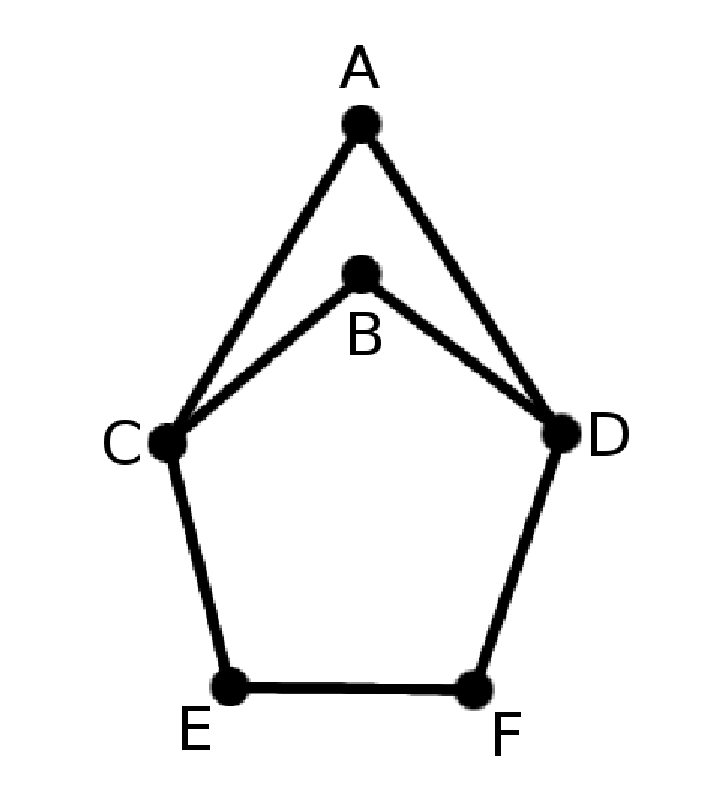
\includegraphics[height=2in]{figures/planar_graph_morning.pdf}
\end{center}

\bparts

\ppart What is its chromatic number? \examrule{0.4in}

\begin{solution}
The graph has an odd length cycle, so its chromatic number must be at least 3. We can find a 3-coloring of the graph (color A, B, and E red, color C and D blue, and color F green), so its chromatic number must be 3.
\end{solution}


\ppart Notice that it's a connected planar graph. Describe all of its discrete faces.

\begin{solution}
Here is one possible answer: \\
ACBDA \\
BDFECB \\
ADFECA \\ \\
These cycles can also be described by rotations of reversals of the sequences. For example, ABCDA can also be expressed as BCDAB or ADCBA (or many other possibilities).
\end{solution}

\eparts

\end{problem}

%%%%%%%%%%%%%%%%%%%%%%%%%%%%%%%%%%%%%%%%%%%%%%%%%%%%%%%%%%%%%%%%%%%%%
% Problem ends here
%%%%%%%%%%%%%%%%%%%%%%%%%%%%%%%%%%%%%%%%%%%%%%%%%%%%%%%%%%%%%%%%%%%%%

\endinput
